\documentclass[male,czech]{kithesis}

\usepackage{graphics}
\usepackage{array}

% zde nastavte základní informace o bakalářské práci
\newcommand{\AUTOR}{Oleg Musijenko}
\newcommand{\TITULcz}{Tacit programming - návrh doménově specifického jazyka a implementace jeho interpretu} % titul v českém jazyce
\newcommand{\TITULen}{Tacit programming - design of a domain specific language and implementation of it's interpreter} % titul v anglickém jazyce
\newcommand{\KLICOVASLOVAcz}{bakalářská práce, odborný text, programování} % klíčová slova v českém jazyce
\newcommand{\KLICOVASLOVAen}{bachelor thesis} % klíčová slova v anglickém jazyce
\newcommand{\VEDOUCI}{Mgr. Jiří Fišer, Ph.D.}    

\newcommand{\PROGRAM}{Aplikovaná informatika}    
\newcommand{\OBOR}{Informační systémy}    

% nastavení fontů (liší se podle TeXovského stroje)
\iftutex
\usepackage{fontspec}
\setmainfont{Libertinus Serif} % použito je opensource písmo Libertinus, lze použít jakékoliv jiné rozumné
\setsansfont{Libertinus Sans}
\setmonofont[Scale = MatchLowercase]{Libertinus Mono}
\usepackage{unicode-math}  
% písmo pro matematiku, vhodná písma viz  	např. https://developer.mozilla.org/en-US/docs/Mozilla/MathML_Project/Fonts
\setmathfont{Libertinus Math}
\else
\usepackage[utf8]{inputenc}
\usepackage[T1]{fontenc}
\usepackage{libertinus}
\usepackage{amsmath,amssymb}
\usepackage{libertinust1math}
\usepackage{graphicx}
\usepackage[font=small, labelfont=bf]{caption}
\fi

\usepackage[style=authoryear,backend=biber,citestyle=nature]{biblatex}
\usepackage{minted}

\addbibresource{bibliografie.bib}
% vylepšení vzhledu
\usepackage{microtype}
%\sloppy %odpoznámkujte pokud vám často přetékají řádky
\renewcommand{\arraystretch}{1.23} % vertikální roztažení tabulek o 23%
            
% nastavení pro sazbu výpisu kódu
\usepackage{listings}

\lstset{ %
  language=Haskell,                % hlavní programovací jazyk, seznam podporovaných viz https://en.wikibooks.org/wiki/LaTeX/Source_Code_Listings
  basicstyle=\ttfamily,    
  showspaces=false,                % show spaces adding particular underscores
  showstringspaces=true,           % underline spaces within strings
  showtabs=false,                  % show tabs within strings adding particular underscores
  frame=single,                    % adds a frame around the code
  tabsize=3,                       % sets default tabsize to 3 spaces
  breaklines=true,                 % sets automatic line breaking
  breakatwhitespace=false,         % sets if automatic breaks should only happen at whitespace
  keywordstyle=\bfseries,          % keyword style
  commentstyle=\rmfamily,          % comment style
  stringstyle=\itshape,            % string literal style
}

% nastavení hypertextových odkazů a PDF metainformací
\usepackage{url} % přidává příkaz url pro sazbu url
\usepackage[unicode=true,colorlinks=true,
            pdftitle={\TITULcz},pdfauthor={\AUTOR},
            pdfkeywords={\KLICOVASLOVAcz}]{hyperref}
            
\pagestyle{fancy} % aktivování stylu záhlaví a zápatí z kithesis

%---------------------------------------------------------

\begin{document}
\thispagestyle{empty}
\begin{center}
{\Huge Univerzita Jana Evangelisty Purkyně \\
v~Ústí nad Labem}
\\[16pt]
{\huge Přírodovědecká fakulta}

\vspace{2cm}
\resizebox{8cm}{!}{
\includegraphics{LOGO_PRF_CZ_RGB_standard.jpg}}

\vspace{2cm}
{
\huge
\TITULcz\par

\vspace{0.5em}
\LARGE\scshape bakalářská práce
}
\end{center} 
 
\vfill
{
\large
\begin{tabular}{>{\bfseries}rl}
    Vypracoval: 	& \AUTOR\\
    Vedoucí práce: 	& \VEDOUCI\\
&\\
Studijní program:       & \PROGRAM\\
Studijní obor:          & \OBOR\\
\end{tabular} 
}
\vspace{1.5cm}
\begin{center}
\Large\scshape   Ústí nad Labem \the\year
\end{center}

\cleardoublepage
\thispagestyle{empty}

\textbf{Zde bude vloženo zadání bakalářské práce!!}

Zadání bakalářské je možné získat až
v okamžiku, kdy je práce schválena ve STAGu vedoucím práce, vedoucím katedry a garantem oboru a nelze tak učinit elektronicky.

Požádejte o něj vedoucího katedry informatiky. Zadání vám bude doporučeno v podobě elektronicky podepsaného PDF, které vložíte na místo toho listu
(dvojstránky) některým z nástrojů pro práci s PDF dokumenty.

\cleardoublepage
\thispagestyle{empty}

\textbf{Prohlášení}

Prohlašuji, že jsem tuto bakalářskou práci vypracoval\ifthenelse{\boolean{feminum}}{a}{} samostatně a použil\ifthenelse{\boolean{feminum}}{a}{}
jen pramenů, které cituji a uvádím v přiloženém seznamu literatury.

\vspace{1em}
Byl\ifthenelse{\boolean{feminum}}{a}{} jsem seznámen\ifthenelse{\boolean{feminum}}{a}{} s tím, že se na moji práci vztahují práva a povinnosti vyplývající ze zákona č. 121/2000 Sb., ve znění zákona č. 81/2005 Sb., autorský zákon, zejména se skutečností, že Univerzita Jana Evangelisty Purkyně v Ústí nad Labem má právo na uzavření licenční smlouvy o užití této práce jako školního díla podle § 60 odst. 1 autorského zákona,s tím, že pokud dojde k užití této práce mnou nebo bude poskytnuta licence o užití jinému
subjektu, je Univerzita Jana Evangelisty Purkyně v Ústí nad Labem oprávněna ode mne požadovat přiměřený příspěvek na úhradu nákladů, které na vytvoření díla vynaložila, a to podle okolností až do jejich skutečné výše.

\vspace{1em}
V Ústí nad Labem dne \today \hspace{0.3\textwidth} Podpis:


\cleardoublepage
\thispagestyle{empty}
~\vfill

\begin{flushright}
  Děkuji vedoucímu práce Mgr. Jiřímu Fišerovi, Ph.D.\\ za neocenitelné rady a pomoc při tvorbě bakalářské práce.
\end{flushright}

\cleardoublepage
\thispagestyle{empty}

\textbf{\textsf{Abstrakt}}

\textsc{\TITULcz}

Abstrakt shrnuje základní motivaci práce (kontext), hlavní cíl a následně jednotlivé
autorské kroky k~jeho splnění (co bylo uděláno od úvodních rešerší, přes návrh, implementaci k případnému nasazení. Minimální rozsah je 800 znaků (maximální půl strany).

\textbf{\textsf{Klíčová slova}}

seznam klíčových slov (obecných termínů vystihujících téma práce) v počtu dva až deset 

\vspace{1em}
\hrulefill
\vspace{1em}

\textbf{\textsf{Abstract}}

\textsc{\TITULen}

Translation of Czech abstract.

\textbf{\textsf{Key words}}

Translation of czech key words.

\tableofcontents

\addchap{Úvod}

Jsou různá programovací paradigmata s kterými se může programátor setkat. Mezi nejznámější 
paradigmata patří strukturované, kde počátek tohoto paradigmatu se datuje v 1967 s Dijkstrovo článkem 
"Goto statement considered harmful". Dijkstra díky 'goto' výrazům nemohl určit správnost programu, proto 
se 'goto' nahradil za struktury typu 'if else', 'while', atd... Poté se můžeme setkat s objektově orientovaným
paradigmatem, který je v dnešní době využíván jak pro menší aplikace, tak pro enterprise systémy. Toto paradigma
dává programátorům možnosti využití polymorfismu, není zapotřebí využívát ukazatele na funkce a pomocí dnešních
nástrojů je jednodušší se zorientovat v zdrojovém kódu. Jako finální paradigma je zde funkcionální. Funkcionální jazyky
omezují primárně omezují mutaci existujících proměnných a zároveň se zaměřují na kompozici funkcí.

Existují samozřejmě i další paradigmata, ale mnohdy je na ně pohlíženo jako na kuriozity. Třeba 
mezi takové patří deklarativní jazyk Prolog, který ověřuje pravdivost výroku v závislosti na předchozích
relací.
Hlavně se budeme zaměřovat na tacit - "beztečkové" paradigma. Do tohoto paradigmatu spadá 
jazyky APL rodiny. Ukážeme si, že i jazyky, které nebyly navržené jako "beztečkové" umožňují v tomto stylu psát.

Tato bakalářská práce předpokládá, že čtenář zná základy funkcionálních jazyků a obzvlášť Haskellu, 
protože návrh je vytvořen v Haskellu pomocí knihoven Parsec a LLVM.

\chapter{Tacit programming}

\textbf{Tacit programming} je styl programování, kde nevyužíváme parametry funkcí, 
místo toho funkce řetězíme, nebo kompozicujeme. Na následujících příkladech v programovacím jazyce
javascript si tento princip ukážeme. 

\begin{minted}{js}
  fetch("APIURL")
  .then(x => fancyFunction(x))
  .then(x => console.log(x))
  .catch(e => throw Error(e))
\end{minted}

Po získání dat provedeme transformaci dat (definice fancyFunction není v tomto kontextu důležitá, stačí pouze vědět, že vrací Promise/Slib) a poté zapíšeme výsledek do konzole. 
Toto je jeden ze způsobů, jak můžeme na sebe řetězit funkce zpětného volání ("Callbacks").

Toto je zcela běžná praxe javascript programátorů, ale bohužel má jednu malou nevýhodu.
Tvoří se zde zbytečná anonymní funkce ("arrow function nebo-li šipková") a pokud bychom prohlubovali čím dál víc 
zásobník volání, mohou nám tyto anonymní funkce zabírat paměť a během debuggingu nám tento styl zápisu "znečišťuje" 
zásobník volání. 

\begin{minted}{js}
  fetch("APIURL")
  .then(fancyFunction)
  .then(console.log)
  .catch(throw Error)
\end{minted}

Zde se nachází kód, který dělá stejné instrukce, jako ten předchozí. Rozdíl je ten, že je zapsán jako \textit{beztečkový - "point free"}.
Takto programátor předchází potřebě dělat obklopující lambda funkce.

Na následujícím přikladě si ukážeme, jak funguje \textbf{currying} a proč souvisí s tacit programováním.

\begin{minted}{js}
const curry = (f) => a => b => f(a,b);

const sayHello = (a, b) = `Hello ${a} from ${b}`;

const applyToFunctionArray = (input,...args) => args.map(a => a(input))

const partiallyAppliedData = ["A", "B", "C"].map(curry(sayHello)); 
// [(b) => "Hello A from ${b}", 
//  (b) => "Hello B from ${b}", 
//  (b) => "Hello C from ${b}"]

const partiallyAppliedData2 = ["A", "B", "C"].map(curry(sayHello)(1)); 
// ["Hello A from 1", 
//  "Hello B from 1", 
//  "Hello C from 1"]
\end{minted}

Curry funkce transfomuje existujícé funkci tak, že máme pro každý argument vlastní vracející funkci. Z 
funkce \textbf{f(a,b,c,d)} vzniká funkce \textbf{f(a)(b)(c)(d)} \cite{Currying}. V čem je toto výhodné?
Například je zde uvedené pole, které se skládá z částečně aplikovaných funkcí. 
Takto může programátor naiterovat odpověď ze serveru do objektu z předchozí ukázky, které je závislé na třeba na uživatelském vstupu. 

Zajímavější část je u \textit{partiallyAppliedData2}. Curryovaná funkce vrací 
funkci, jež očekává vstupní parametr, aby byla vyhodnocena. Tento princip je důležitý
pro lenivé vyhodnocení, který využívá Haskell.

Může zde padnout argument, že v našem případě se curryování nachází pouze pro funkci,
která prijímá dva argumenty. Zde je definice funkce, která převádí jakoukoliv funkci na curryovanou.

\begin{minted}{js}
const curry = (f) => (..args) => args.length >= f.length ? 
  f.apply(this, args) : (...args2) => curry.apply(this, args.concat(args2));
\end{minted}

\section{Principy a odlišnosti od klasického procedurálního paradigmatu}

Procedurální paradigma se zaměřuje na psaní procedurálních instrukcí.
Typickým příkladem tohoto paradigmatu je programovací jazyk C, protože se
jedná o standard, tak v následujících příkladech budu porovnávat jazyk C s jazykem Haskell.
Haskell je primárně funkcionální jazyk, tento jazyk nám umožňujě psát funkce
v "beztečkovém" stylu. 

Ukažme si následující příklad sumace.

\textbf{Haskell}
\begin{minted}{Haskell}

sumCustom:: (Traversable t, Num a) => t a -> a
sumCustom = foldr (+) 0

\end{minted}

\pagebreak

\textbf{C}
\begin{minted}{C}
int sum(int* arr, size_t numOfElements)
{
    int acc = 0;
    
    for(int i = 0; i < numOfElements; i++)
    {
        acc += *(arr + i);
    }
    
    return acc;
}
\end{minted}

Na příkladu jde vidět, že beztečkový styl zápisu je opravdu kompaktní. 
V Haskellu vůbec neinteragujeme s parametry funkce.
Tento příklad je založen na podstatě tacit programmingu.
Co se týče algoritmizace, tacit programming je známý pro vytváření 
algoritmických řešení pomocí pouze jednoho řádku kódu. 


Na dalším příkladě si ukážeme fibonnacciho posloupnost.

\textbf{Haskell}
\begin{minted}{Haskell}
-- Využijeme lenivosti haskellu a vytvoříme nekonečnou 
-- posloupnost fibonacciho čísel

fibonacci:: Num a => Int -> [a]
fibonacci = (flip take) fibonacciInfinite
  where
    fibonacciInfinite:: Num a => [a]
    fibonacciInfinite = scanl (+) 0 (1:fibonacciInfinite)

\end{minted}

\pagebreak

\textbf{C}
\begin{minted}{C}

void fibonacci(int* arr, size_t numOfElements)
{
    if(numOfElements > 0)
    {
      arr[0] = 0;
    }
    if(numOfElements > 1)
    {
      arr[1] = 1;
    }
    for(int i = 2; i < numOfElements; i++)
    {
      arr[i] = arr[i - 1] + arr[i - 2];
    }
}

\end{minted}

Z pohledu imperativního programátora implementace v C je zcela jasná. Funkce přijímá ukazatel na
pole a modifikuje toto pole. Zatímco v Haskellu tato implementace může být matoucí. Funkce scanl je 
velice podobná funkci foldl, jen místo vracení akumulátoru, tak vrací průběžně vypočtené hodnoty.

\section{Rešerše existujících implementací}

\chapter{DSL - principy a využití}
DSL (Domain Specific Language) jsou jazyky, které se zaměřují na specifickou doménu problematiky.
Obecně DSL jazyky jsou mnohem jednodušší než jejich plnohodnotné protějšky. Výhodou je, že 
křivka učení je o mnohem nižší než u GPL (General Purpouse Language). Zároveň pokud potřebujete
na dannou práci experty z oboru, jako jsou například doktoři nebo architekti, tak ty nepotřebují znát detaily 
implementace algoritmů, ale místo toho pokud budou mít přístup rovnou k DSL - šikmost stěny,
hodnota cukrů v krvi pacienta, tak mohou plnit svojí práci o mnohem efektivněji. \cite{DomainSpecificLanguages}

Jedním z takových typických jazyků je \textbf{HTML a CSS}. HTML se zaměřuje na vytvoření rámce pro zobrazení textu,
zatímco CSS se zaměřuje na stylizaci webu pomocí DOM selectorů. Pravdou je, že pro CSS se nenachází žádný 
protocol a proto v různých webových enginech, můžete dostat různé výsledky. Příkladem z praxe je zpracování
fontů.

Též existují jazyky DSL, které jsou specifické pouze pro jednu dannou enterprise aplikaci, kde její implementace
často spočívá na bázi XML nebo podobného formátu jako je např YAML. Zde DSL slouží například pro 
zjednodušení UI nebo business logiky. Třeba pro porovnání \textbf{XAML} pro .NET platformu zjednodušuje logiku, 
stylizuje UI a zároveň zbavuje potřeby tvoření "glue" kódu.

Další jazyk který je velice využíván v hardwarovém prostředí je \textbf{VHDL} nebo \textbf{Verilog}. Tyto DSL jsou zaměřená
na simulaci obvodů pomocí FPGA (hradlových polí). Pro building C/C++ projektů existuje \textbf{makefile}. Jedním ze zajímavějších
DSL je DSL pro "continuous integration and deployment". Různé firmy co nabízejí online repositáře se v tomto budou trochu lišit, ale
většina z nich poskytují jakousi formu automatizaci deploymentu. Toto poskytují firmy jako je GitHub,
GitLab nebo Azure Dev Ops. Na GitHubu pomocí YAMLu můžete sepsat instrukce na testování a deployment aplikace.

\pagebreak
\centering
\captionof{figure}{Výstřižek z GitHub Actions}
\resizebox{15cm}{!}{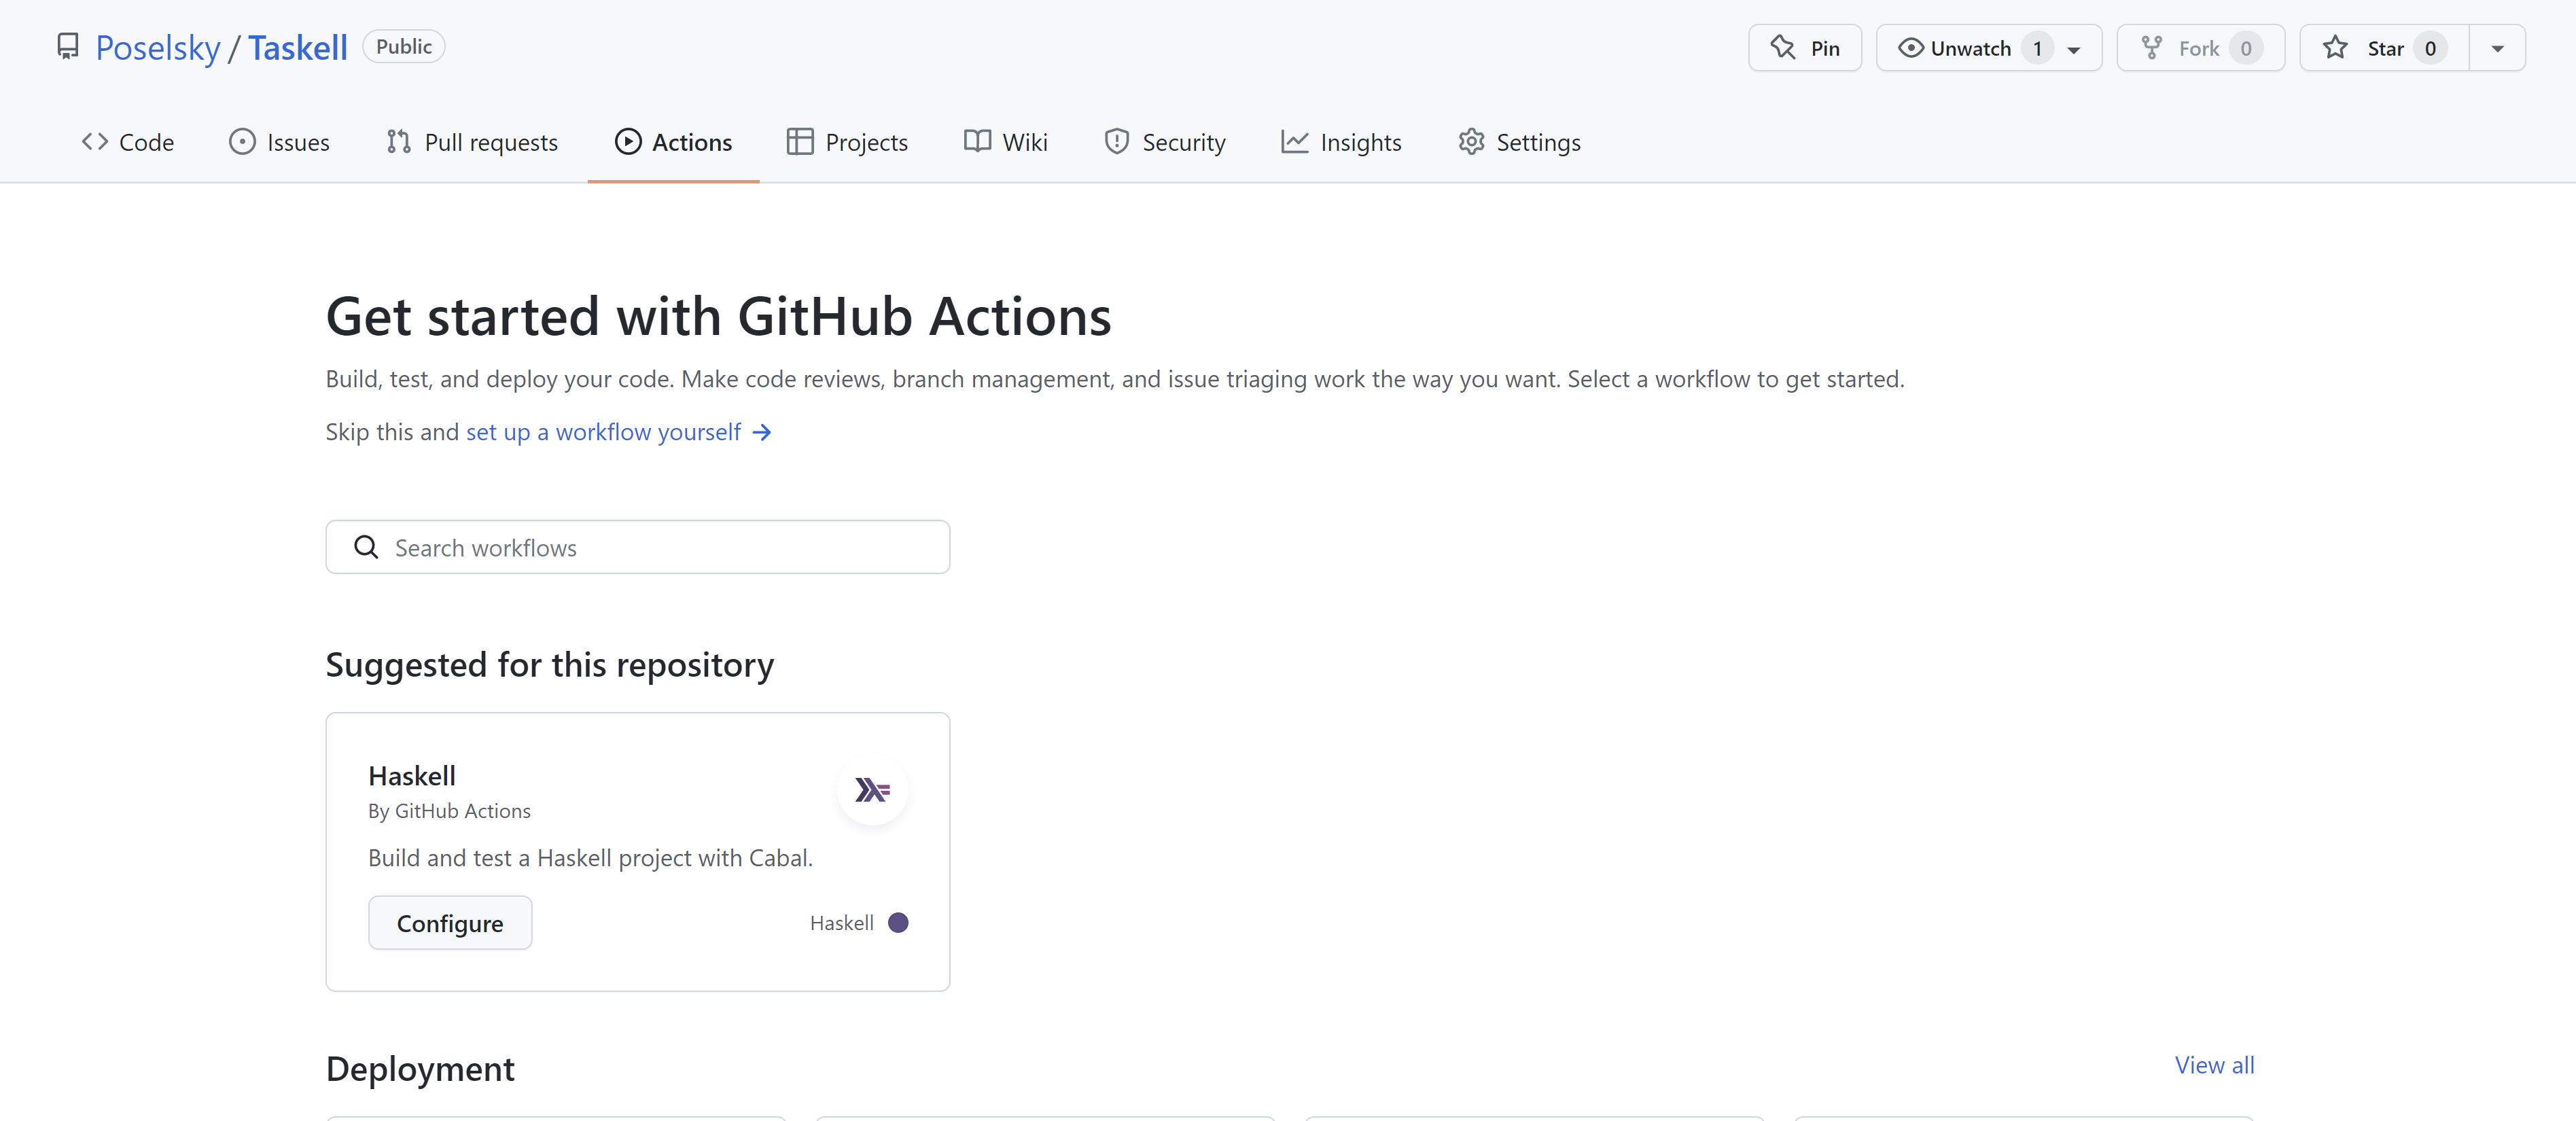
\includegraphics{Deployment.PNG}}

\chapter{Návrh vlastního DSL}
Pro návrh jsem zvolil programovací jazyk Haskell. 

\chapter{Implementace interpretu navrženého DSL}

\chapter{Ověření použitelnosti (testování funkčnosti, praktické příklady využití)}

\chapter{Závěr}

\chapter{Citace}


\cite{Katuscakc}
\cite{IntroToLLVM}
\printbibliography


\appendix




\end{document}